% !TEX program = xelatex
\documentclass[UTF8]{ctexart}
\usepackage{tikz}
\usepackage{amsmath}
\usepackage{amssymb}


\begin{document}
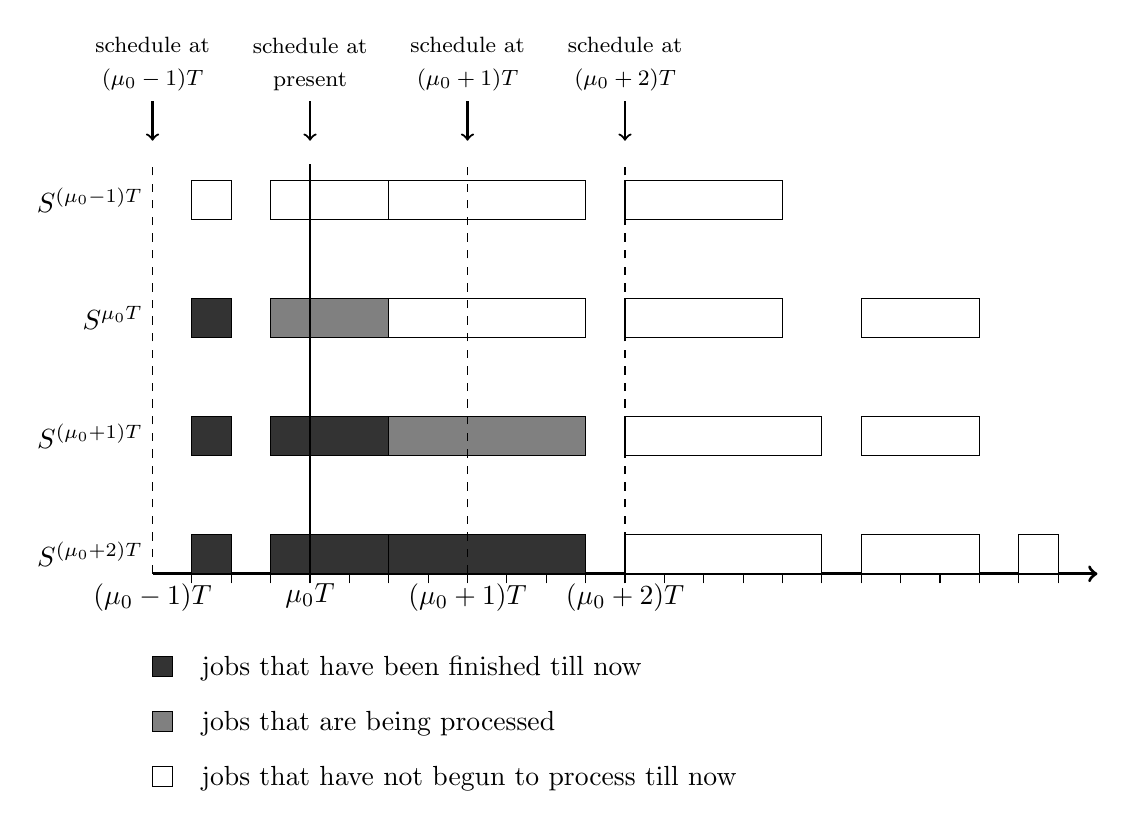
\begin{tikzpicture}[scale = 1]
	\draw [->] [very thick] (-2, 0) -- (10, 0);
	\foreach \x in {-1.5, -1, ..., 9.5}
		\draw (\x, -3.5pt) -- (\x, 3.5pt);

	\filldraw [fill = white] (-1.5, 4.5) rectangle +(0.5, 0.5);
	\filldraw [fill = white] (-0.5, 4.5) rectangle +(1.5, 0.5);
	\filldraw [fill = white] (1, 4.5) rectangle +(2.5, 0.5);
	\filldraw [fill = white] (4, 4.5) rectangle +(2, 0.5);

	\filldraw [fill = white!20!black] (-1.5, 3) rectangle +(0.5, 0.5);
	\filldraw [fill = gray] (-0.5, 3) rectangle +(1.5, 0.5);
	\filldraw [fill = white] (1, 3) rectangle +(2.5, 0.5);
	\filldraw [fill = white] (4, 3) rectangle +(2, 0.5);
	\filldraw [fill = white] (7, 3) rectangle +(1.5, 0.5);

	\filldraw [fill = white!20!black] (-1.5, 1.5) rectangle +(0.5, 0.5);
	\filldraw [fill = white!20!black] (-0.5, 1.5) rectangle +(1.5, 0.5);
	\filldraw [fill = gray] (1, 1.5) rectangle +(2.5, 0.5);
	\filldraw [fill = white] (4, 1.5) rectangle +(2.5, 0.5);
	\filldraw [fill = white] (7, 1.5) rectangle +(1.5, 0.5);

	\filldraw [fill = white!20!black] (-1.5, 0) rectangle +(0.5, 0.5);
	\filldraw [fill = white!20!black] (-0.5, 0) rectangle +(1.5, 0.5);
	\filldraw [fill = white!20!black] (1, 0) rectangle +(2.5, 0.5);
	\filldraw [fill = white] (4, 0) rectangle +(2.5, 0.5);
	\filldraw [fill = white] (7, 0) rectangle +(1.5, 0.5);
	\filldraw [fill = white] (9, 0) rectangle +(0.5, 0.5);

	\draw [dashed] (-2, 0) -- (-2, 5.2);
	\draw (0, 0) -- (0, 5.2);
	\draw [dashed] (2, 0) -- (2, 5.2);
	\draw [dashed] (4, 0) -- (4, 5.2);
	\draw [->] [thick] (-2, 6) node [anchor = south, align=center] {\footnotesize schedule at \\ \footnotesize $(\mu_0 - 1)T$} -- (-2, 5.5);
	\draw [->] [thick] (0, 6) node [anchor = south, align=center] {\footnotesize schedule at \\ \footnotesize present} -- (0, 5.5);
	\draw [->] [thick] (2, 6) node [anchor = south, align=center] {\footnotesize schedule at \\ \footnotesize $(\mu_0 + 1)T$} -- (2, 5.5);
	\draw [->] [thick] (4, 6) node [anchor = south, align=center] {\footnotesize schedule at \\ \footnotesize $(\mu_0 + 2)T$} -- (4, 5.5);

	\draw (0, 0) node [anchor = north] {$\mu_0 T$};
	\draw (-2, 0) node [anchor = north] {$(\mu_0 - 1)T$};
	\draw (2, 0) node [anchor = north] {$(\mu_0 + 1)T$};
	\draw (4, 0) node [anchor = north] {$(\mu_0 + 2)T$};

	\draw (-2, 4.75) node [anchor = east] {$S^{(\mu_0 - 1)T}$};
	\draw (-2, 3.25) node [anchor = east] {$S^{\mu_0 T}$};
	\draw (-2, 1.75) node [anchor = east] {$S^{(\mu_0 + 1)T}$};
	\draw (-2, 0.25) node [anchor = east] {$S^{(\mu_0 + 2)T}$};

	\filldraw [fill = white!20!black] (-2, -1.3) rectangle +(0.25, 0.25);
	\draw (-1.5, -1.2) node [anchor = west] {jobs that have been finished till now};
	\filldraw [fill = gray] (-2, -2) rectangle +(0.25, 0.25);
	\draw (-1.5, -1.9) node [anchor = west] {jobs that are being processed};
	\filldraw [fill = white] (-2, -2.7) rectangle +(0.25, 0.25);
	\draw (-1.5, -2.6) node [anchor = west] {jobs that have not begun to process till now};
\end{tikzpicture}

\begin{tikzpicture}
\filldraw [fill opacity = 0] (0, 0) rectangle +(12, 5);
\draw (1, 3) circle (0.15);
\draw [->] (1.15, 3) -- (1.65, 3);
\draw (1.8, 3) circle (0.15);
\draw [->] (1.95, 3) -- (2.45, 3);
\draw (2.6, 3) circle (0.15);
\draw [->] (-60: 0.15cm) ++(1.8, 3) -- +(0.25, -0.433);
\draw (-60: 0.8cm) ++(1.8, 3) circle (0.15);
\draw [->] (-60: 0.8cm) ++(1.95, 3) -- +(0.5, 0);
\draw (-60: 0.8cm) ++(2.6, 3) circle (0.15);
\draw [->] (-60: 0.15cm) ++(2.6, 3) -- +(0.25, -0.433);

\end{tikzpicture}

\begin{table}[tb]
	\caption{sky is sb}
	\label{tab:tablename}
	\centering

	\begin{tabular}{ll}
	\hline

	\hline
	\textbf{Sets} & \textbf{Descriptions} \\
	\hline
	$\mathcal{N}_i$ & \text{set of operations of job $i$; $j \in \mathcal{N}_i$} \\
	$\mathcal{I}$ & \text{set of jobs; $i \in \mathcal{I}$} \\
	$\mathcal{K}$ & \text{set of services; $k \in \mathcal{K}$}\\
	\hline
	\textbf{Parameters} & \textbf{Descriptions} \\
	\hline
	$\lambda_{ijk}$ & \text{whether operation $j$ of job $i$ can be processed on service $k$} \\
	$s_{ij}$ & \text{start time of operation $j$ of job $i$} \\
	$c_{ij}$ & \text{completion time of operation $j$ of job $i$} \\
	$p_{ij}$ & \text{processing time of operation $j$ of job $i$} \\
	$M$      & \text{a sufficently large positive integer} \\
	\hline

	\hline
	\end{tabular}
\end{table}



\begin{equation}
x_{ijk} := 
\begin{cases}
1, & \text{if operation $j$ of job $i$ is allocated to service $k$}, \\
0, & \text{otherwise}.
\end{cases}
\end{equation}

\begin{equation}
y_{iji^{'}j^{'}k} := 
\begin{cases}
1, & \text{if operation $j$ of job $i$ is processed before operation $i^{'}$ of job $j^{'}$ on service $k$}, \\
0, & \text{otherwise}.
\end{cases}
\end{equation}

\begin{equation}
z_{ijl} := 
\begin{cases}
1, & \text{if operation $l$ of job $i$ is processed after operation $j$ of job $i$}, \\
0, & \text{otherwise}.
\end{cases}
\end{equation}

\begin{equation}
\text{minimize} \quad \max \sum_{i \in \mathcal{I}, k \in \mathcal{K}} c_{ijk},
\end{equation}

\begin{align}
\text{subject to} \quad \sum_{k \in \mathcal{K}} x_{ijk} = 1, &\quad j \in \mathcal{N}_i, i \in \mathcal{I}, \\
x_{ijk} \leqslant \lambda_{ijk}, &\quad j \in \mathcal{N}_i, i \in \mathcal{I}, k \in \mathcal{K},\\
y_{iji^{'}j^{'}k} + y_{i^{'}j^{'}ijk} \leqslant x_{ijk}, &\quad j \in \mathcal{N}_i, j^{'} \in \mathcal{N}_{i^{'}}, i, i^{'} \in \mathcal{I},  (i, j) \ne (i^{'}, j^{'}), k \in \mathcal{K},\\
y_{iji^{'}j^{'}k} + y_{i^{'}j^{'}ijk} + 1 \geqslant x_{ijk} + x_{i^{'}j^{'}k}, &\quad j \in \mathcal{N}_i, j^{'} \in \mathcal{N}_{i^{'}}, i, i^{'} \in \mathcal{I},  (i, j) \ne (i^{'}, j^{'}), k \in \mathcal{K},\\
s_{ij} + p_{ij} - M(1 - y_{iji^{'}j^{'}k}) \leqslant s_{i^{'}j^{'}}, &\quad j \in \mathcal{N}_i, j^{'} \in \mathcal{N}_{i^{'}}, i, i^{'} \in \mathcal{I},  (i, j) \ne (i^{'}, j^{'}), k \in \mathcal{K},\\
s_{ij} + p_{ij} \leqslant z_{ijl}s_{il}, &\quad j, l \in \mathcal{N}_i, i \in \mathcal{I}, j \ne l, \\
s_{ij} \geqslant 0, &\quad j \in \mathcal{N}_i, i \in \mathcal{I}, \\
x_{ijk} \in \{0, 1\}, &\quad j \in \mathcal{N}_i, i \in \mathcal{I}, k \in \mathcal{K}, \\
y_{iji^{'}j^{'}k} \in \{0, 1\}, &\quad j \in \mathcal{N}_i, j^{'} \in \mathcal{N}_{i^{'}}, i, i^{'} \in \mathcal{I},  (i, j) \ne (i^{'}, j^{'}), k \in \mathcal{K},\\
z_{ijl} \in \{0, 1\}, &\quad j, l \in \mathcal{N}_i, i \in \mathcal{I}, j \ne l,
\end{align}


\end{document}